%! Author = alida
%! Date = 20/11/2024

% Preamble
\documentclass[@SRC@/main]{subfiles}

% tutti i pacchetti usati vanno nel main

% Document
\begin{document}
\clearpage
\section{Analisi}

\begin{center}
\begin{minipage}{.8\textwidth}
  \centering
  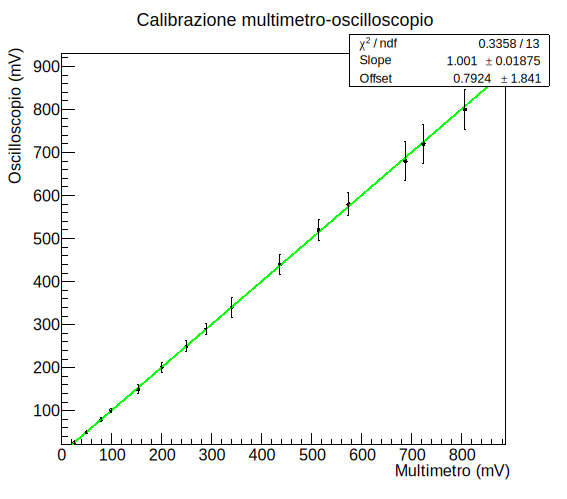
\includegraphics[width=.75\textwidth]{calibrazione.png} 
  \captionof{figure}{Grafico e fit dei valori ottenuti dalla misura di calibrazione}
  \label{fig:calibrazione}
\end{minipage}
\\
\begin{minipage}{.95\textwidth}
  \centering
  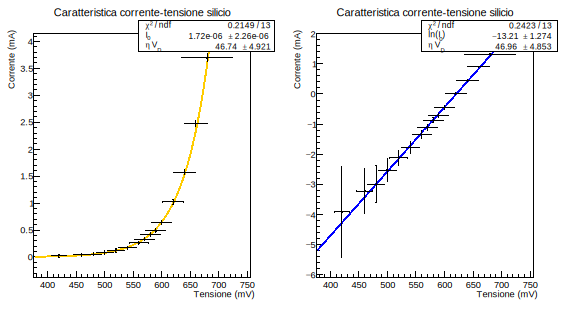
\includegraphics[width=\textwidth]{silicio.png} 
  \captionof{figure}{schematizzazione della struttura del disco, nella prima figura visto dall'alto, nella seconda met\`a di una sezione frontale.}
  \label{fig:silicio}
\end{minipage}
\\
\begin{minipage}{.95\textwidth}
  \centering
  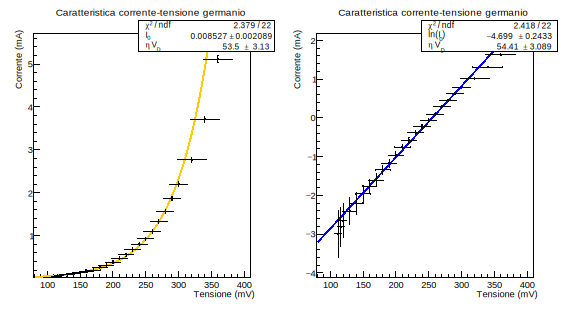
\includegraphics[width=\textwidth]{germanio.png}
  \captionof{figure}{schematizzazione della struttura del disco, nella prima figura visto dall'alto, nella seconda met\`a di una sezione frontale.}
  \label{fig:germanio}
\end{minipage}
\end{center}

\end{document}